%!TEX root = gutter+stars.tex

%%%%%%%%%%%%%
%%%%%%%%%%%%%
%%%%%%%%%%%%%
%%%%%%%%%%%%%
%%%%%%%%%%%%%
%%%%%%%%%%%%%
%%%%%%%%%%%%%
%%%%%%%%%%%%%

\chapter{User Study on API Learning}
\label{the chapter on the MSR user study}

Modern software development requires a large investment in learning application programming interfaces (APIs).
%
Recent research found that the learning materials themselves are often inadequate: developers struggle to find answers beyond simple usage scenarios.
%
Solving these problems requires a large investment in tool and search engine development.
%
To understand where further investment would be the most useful, we ran a study with 19 professional developers to understand what a solution might look like, free of technical constraints. In this chapter, we report on design implications of tools for API learning, grounded in the reality of the professional developers themselves. 
The reoccurring themes in the participants' feedback were trustworthiness, confidentiality, information overload and the need for code examples as first-class documentation artifacts.

Modern application programming interfaces (APIs) allow developers to reuse existing components. API learning is a continuous process. Even when a developer makes a large initial investment in learning the API, 
for example, by reading books or going through online tutorials, 
the developer will continue to consume online material 
about the API 
throughout the development process. These materials include reference documentation from the API provider, sample code, blog posts, and forum questions and answers. 

Indeed, seeking online API information has become such a pervasive part of modern programming that emerging research tools blend the experiences of the browser and the development environment. For example, Codetrail automatically links source code and the web pages viewed while writing the code \cite{gm09}. Blueprint allows a developer to launch a web query from the development environment and incorporate code examples from the resulting web pages \cite{bdwk10}. While these new tools help reduce the cost of (re)finding relevant pages and incorporating information from them, this addresses only a portion of developers' frustrations. 
%
In a recent study of API learning obstacles among professional developers, Robillard found that the learning materials themselves are often inadequate~\cite{robillard09}. Bajracharya and Lopes analysed a year's worth of search queries and found that current code search engines address only a subset of developers needs~\cite{Bajracharya2009a}.   
For example, developers struggled to find code examples beyond simple usage scenarios, to understand which parts of an API support which programming tasks, and to infer the intent behind the API's design. 
Solving these systematic problems requires a large investment, either in the API provider's official documentation, the API users' community-based documentation, or in the search engines that unite the two \cite{bdwk10,Hoffmann2007a}. 
%Where should such an investment be made? Should API providers create more extensive documentation on complex usage scenarios and design intent? Should the API users push for mass organization of content based on tagging or wikis? Should search engines create more sophisticated indices of API web pages, e.g. by parsing embedded code snippets? 
Any of these changes is difficult and expensive.

% NOTE: I originally anonymized "Microsoft" and "Silverlight" but it seemed a bit silly.

To understand where further investment would be the most useful, we ran a study with 19 professional developers from Microsoft Corporation, with the goal of understanding what an ``ideal'' solution might look like, free from technical constraints. We invited randomly chosen members of a corporate email list of  Silverlight users to participate in one-hour sessions for small gratuities. Silverlight is a large API for creating web applications, with hundreds of classes for data persistance, data presentation, and multimedia. All participants were male with an average of $12.2$ years of professional experience. 

Borrowing from participatory design, we asked the participants to act as our partners in designing a new user experience for learning Silverlight. We ran two types of sessions.  In the first, we interviewed participants to learn their common learning materials and  most challenging learning tasks and then asked them to sketch a design for a new learning portal. We compiled these ideas into five exploratory designs. In the second type of session, we ran focus groups to get feedback on our descriptions of their learning tasks and the five designs. 

This chapter's main contributions are a compilation of design implications for API learning tools, grounded in the reality of the professional developers themselves. We report on the recurring themes in the participants' feedback: trustworthiness, confidentiality, information overload and the need for code examples as first-class documentation artifacts.

\begin{figure*}
    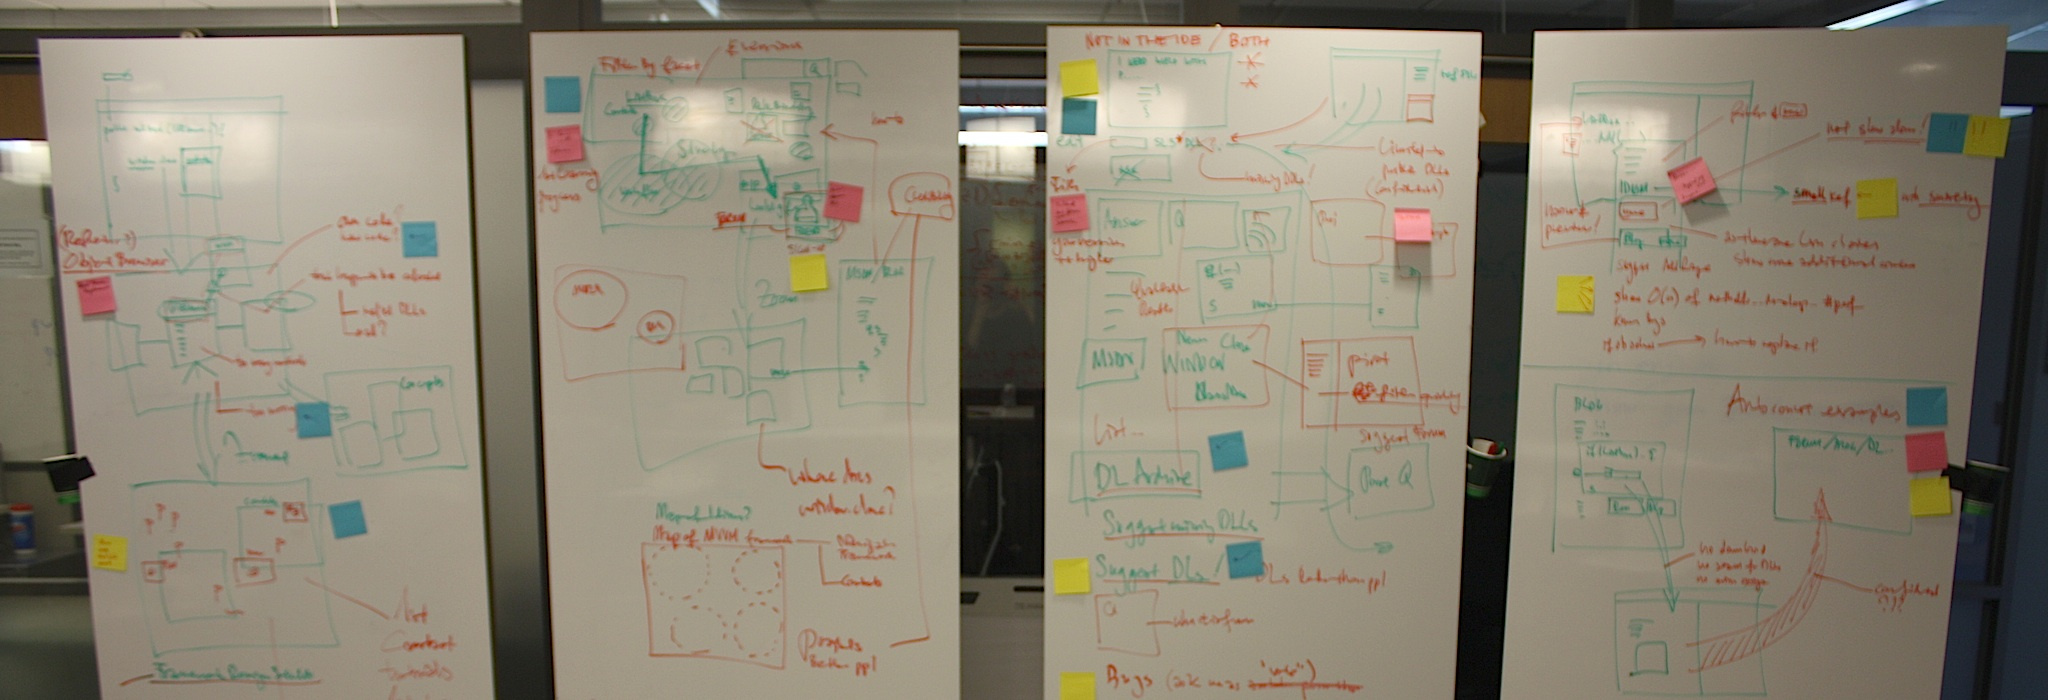
\includegraphics[width=\linewidth]{fig/api-learning-five-design}
    \caption{The five solution designs as narrated to the participants (from left to right): \ZoomableUML, \ConceptMap, \FacettedSearch, and on the last panel \RichIntellisense~(above) and \CloudREPL~(below). Pen color has been used to distinguish the designs (green) from the participant's input (red). The stick notes are the participant's votes.}
    \label{fivedesigns}
\end{figure*} 

\moarsauce
\section{First Study: Current Practice}

In the first type of study session, we met singly with nine participants, and ran each through three activities. First, we asked the participant to describe all the  materials he used for learning Silverlight, as we recorded them on the whiteboard. Next, we asked him to consider this as a set of ``ingredients'' and to sketch a design for a learning portal that presents some or all of these ingredients to help developers learn Silverlight. Finally, we asked him to review the design by comparing the experience of learning Silverlight by using the design versus his own experience learning Silverlight.

\moarsauce
\subsection{Learning Sources}
We asked the participant to describe all the  materials he used for learning Silverlight, as we recorded them on the whiteboard. Some of the learning sources are obvious and readily reported by participants, such as books and web search. To learn about non-obvious learning sources, we asked developers ``did you ever find an answer to a technological question that is not listed here,'' which led to answers like reverse engineering or social networking. Their reported learning sources are the following:

\begin{description}
\item[``Off the top of my head''] is by far the most common way developers find answers on the job. Most participants reported that they set aside dedicated time for learning. Typical off-the-job learning sources are: lurking on mailing lists and forums, watching videos and reading books. Most knowledge however is based on experience and acquired through learning-by-doing on the job. One participant refers to this a \emph{``growing your own folklore.''}

\item[Web search] was reported by all participants as the first place to go when they have an information need. Among the search results participants are typically looking for are: blog posts, discussion forums, official reference documentation, mailing list archives, bug reports and source repositories (listed in order of typical access patterns). 
Participants prefer results with code examples over results without code examples, which is supported by existing research on API learning barriers \cite{robillard09}.

\item[Intellisense] (\ie auto-completion of identifiers) was reported as a tool for the discovery of unknown APIs by all developers. One participant called this \emph{``digging through the namespaces.''} Discovering unknown APIs is an appropriation of auto-completion, originally conceived to help recall names from familiar APIs. 

\item[Prototyping,] reverse engineering and many more forms of tinkering were reported by all participants as a last resort when all above sources failed to provide an answer. 
Some participants even resort to reverse engineering when documentation is available, as they prefer source code over natural language documentation. 
Developers typically use prototyping both as an explorative tool and to verify hypotheses about the APIs. All participants reported that having to \emph{``get your hands dirty''} is an integral part of their learning experience. 

\item[Asking another person] was reported by most participants as a last resort. Developers follow a ``due diligence'' process before asking another person for an answer. It is important to them to have put enough personal effort into finding an answer before asking on a mailing list or reaching out to a person from their social network. 
Also, they reported to prefer immediate results, such as those provided by web search, over waiting for the reply of asynchronous communication such as email and discussion forums.

\end{description}

These findings are consistent with Robillard's study of learning obstacles~\cite{robillard09}, but provide a more complete catalog of learning materials. Both studies found that developers strive to stay within the programming patterns and use cases that the API provider intends (even when that intent is undocumented) and that developers typically lack documentation when using an API for a less common task. Somewhat surprisingly, we found that developers prefer the community-based learning materials on the web, like blogs, forum posts, and tutorials, over more ``authoritative'' learning material, like books and reference documentation. Developers also prefer active but potentially time-consuming information seeking,~like iterative web search and reverse engineering, to waiting for answers from others, because they perceive the answers as more immediate.

\moarsauce
\subsection{Learning Categories}

% renamed this to learning categories, since "task categories" might be confused by reviewers with tasks in a suer study (at least Niko was clearly confused when reading this draft!) 

Based on the design sketches that participants produced, we elicited three broad categories of learning tasks:

\begin{description}
\item[Technology selection] is about learning about an API's fundamental capabilities (\emph{``Can Silverlight play video in this codec?''}) and about comparing capabilities (\emph{``Is DirectX or Silverlight better for my game?''}). Sometimes the selection decision is about growing skills rather than project requirements. 

\item[Mapping task to code] includes both discovery of unfamiliar APIs as well as remembering relevant identifier names in previously learned APIs. Getting an answer to this type of questions typically falls in two phases. Initially developers search based on natural language task descriptions (e.g. \emph{``how to implement a zoomable canvas''}) and skim through many search results to stumble on relevant identifier names. Once they have a concrete identifier, their search behavior becomes more focused and may be as simple as looking up the identifier's reference documentation.

\item[Going from code to better code] is a major concern of professional developers. All participants reported that they spend considerable effort getting answers to performance questions. Other use cases are robustness and idiomatic, \ie intended, use of an API, in particular with regard to breaking changes of newly released API versions or different target platforms.

\end{description}

The kind of learning categories impacts the preferred learning sources and strategies of developers. For technology selection, participants sometimes use web search to learn about available technologies, but eventually prefer personal recommendations from their social network.  For mapping task to code, participants strongly prefer search results with code examples over those without code examples. For getting to better code however, such as troubleshooting a performance problem, participants prefer solving the problem themselves (including reverse engineering) but sometimes ask others to double-check the answers they find.

\moarsauce
\section{Second Study: Solution Elements}

For the second type of session, we compiled the user feedback from the first sessions into five exploratory designs. We ran 10 participants in three focus groups (with three, three, and four members) and asked them to provide feedback on the five designs. In each session, we drew each design on its own whiteboard and encouraged participants to ask questions, provide feedback, and to add their own ideas as we explained the design. 

Figure~\ref{fivedesigns} shows a photograph of the whiteboards with the five designs, taken at the end of a focus group's session. In the following the designs are described in the order they were presented to the participants in that session:

\moarsauce
\paragraph{Design: \ZoomableUML} 
This design draws from the spatial software representation of CodeCanvas~\cite{Deline2010a} and addresses answering complex reachability questions~\cite{Latoza2010a} as you code. The design extends the IDE with a zoomable UML diagram. The diagram opens zoomed on locally reachable types of the API and shows their dependencies and interaction. The user can zoom out to get a larger picture of the API, up to the level of namespaces.

\moarsauce
\paragraph{Design: \ConceptMap} 
The API is presented as a zoomable map, organized around programming domain concepts (e.g. ``controls'', ``media content''). As the user zooms in, the concepts become more refined (e.g. ``streaming video''). At the lowest zoom level, the map shows web-based content about that concept, including blogs, forum posts, tutorials, and the people who author these.
The map is searchable and keeps track of user interaction as well as the user's learning progress. Users can bookmark locations and share their bookmarks. Documentation editors can use the same feature to share tutorials as ``sight-seeing tours.''

\moarsauce
\paragraph{Design: \FacettedSearch}
This design unifies web search and asking people questions. The user types a question into a textbox. As she types, related  search results are pulled in from various sources (web sites, bug reports, code examples, mailing list archives, etc). Search results are grouped by facets, such as type of sources, type of content or semantic concepts. Besides the results, a tag cloud appears with extracted identifier names. Search results are summarized using code examples, if possible. In addition, the results include suggested people and mailing lists that are experts on the topic of the questions, to which the question can be posted.

\moarsauce
\paragraph{Design: \RichIntellisense} 
This design extends auto-completion of identifiers with search results that are automatically pulled from the world wide web. The results are ``localized'' to the current context of the IDE, such as imported libraries and reachable types \cite{Holmes2005}. Results are shown in the same pop-up windows as the auto-completion suggestions. If possible, search results are displayed as code examples ready for incorporating into the code, as in Brandt et al \cite{bdwk10}.

\moarsauce
\paragraph{Design: \CloudREPL} 
This design attaches an execution context to code examples on the web. Code examples include hidden meta-information with all context that is required to execute. Examples are editable, debuggable and can be executed live in the browser. With a single click, users can download examples into their IDEs. Similarly, users can upload the code in their IDE as runnable examples on the web, for inclusion in blogs or discussion forums.

\moarsauce
\section{Feedback}

After we explained all five designs, we then handed each participant a pen and sticky notes and gave them 10 minutes to annotate the designs, either with a blank sticky note to mean ``I like this part'' or with their own comments (typical ones were smiley faces, frowny faces, ``NO'', etc). 

The votes are summarized in Table~\ref{thetable}: the most popular designs are ``\FacettedSearch'' and for learning activities the ``\ConceptMap'' design. Participants downvoted the ``\ZoomableUML'' and ``\RichIntellisense'' due to concerns about information overload, the same happening with ``\CloudREPL`` due to concerns about missing confidentiality.

\begin{table}[h]
\begin{center}
\begin{tabular}{l|ll}
\textbf{Design} & Up-Votes & Down-Votes \\
\hline
\ZoomableUML & $\star\star\star\star~$ & $\ast\ast\ast\ast\ast~$ \\
\ConceptMap & $\star\star\star\star\star\star~$ & $\ast\ast\ast~$ \\
\FacettedSearch & $\star\star\star\star\star\star\star\star\star~$ & $\ast~$ \\
\RichIntellisense & $\star\star\star~$ & $\ast\ast\ast\ast\ast\ast\ast~$ \\
\CloudREPL & $\star\star\star~$ & $\ast~$
\end{tabular}
\end{center}
\caption{At the end of the second type of sessions, participants voted with sticky notes for the designs. \FacettedSearch{} received the most up votes, \RichIntellisense{} the most down votes.}
\label{thetable}
\end{table}%

There were several recurring themes in our participants' feedback which cut across the various designs. The four top-most recurring themes are discussed and summarized as design implications for tool builders in the following:

\moarsauce
\subsection{Code Examples}

We got very positive feedback on the emphasis on code examples and identifier names in the ``\FacettedSearch'' design. Participants prefer results with code examples over results without code examples, which is supported by existing research on API learning barriers \cite{robillard09}. When mapping a task to code, developers typically use web search and linearly go through all results until they find one with a code example or an identifier; often repeating this process a dozen times until they find a working answer. Participants liked about the facetted search design that it extracts code examples and identifiers from top search results. One participant even said that the summary tag cloud with identifiers, by itself, would be reason to use it.

\emph{Implication for tool builders:} Developers need the heterogeneous learning materials that web search provides, but want it to be more targeted and organized. Search engines for API learning should extract code examples and identifiers found in natural text documents, and present them to the developers in a more accessible way. This implication is supported by related work on code examples \cite{bdwk10,Hoffmann2007a,Holmes2005}.

\moarsauce
\subsection{Credibility}

Credibility of web sources appeared as a major concern with all designs that included content taken from the web. For the participants, credibility is mostly a function of where the information comes from. For example, participants reported that search results from blogs are often more relevant, but typically less credible than official reference documentation. They also rely on the social reputation of its source rather than technical factors, which supports existing research \cite{Gysin2010a}. In particular with the ``\FacettedSearch'' design, which automatically summarizes search results, participants emphasized the importance of seeing the information source to judge credibility.  

\emph{Implication for tool builders:} Tools should show both credibility and relevance when presenting search results, so that the developers can make an informed decision when using API information and code examples from the web. To assess the credibility of API information tools should prefer social factors, such as the credibility of the information's author, rather than technical statistics, such as code metrics.

\moarsauce
\subsection{Confidentiality}

Confidentiality appeared as a major concern with all designs that share local information with a global audience. In particular with the ``\CloudREPL'' design, which publishes an example's execution context on the web, participants were concerned with leaking proprietary information, like the use of certain libraries. One participant was also concerned that publicly inquiring about technologies could accidentally reveal business strategies.

\emph{Implication for tool builders:} When automatically sharing local information with the web, tools must be careful to protect proprietary information, such as confidential code and libraries being used. Tools should give developers full control over shared information, for example by letting them review the list of automatically included terms before issuing the search query. Or alternatively, only sharing information that is on a user controlled white list.

\moarsauce
\subsection{Information Overload} 

Information overload was the major reason why participants rejected the ``\ZoomableUML'' and the ``\RichIntellisense'' designs. We got strong feedback that pulling more information into the IDE is not welcome unless it is highly task- and context specific. Participants were also concerned that adding more features to Intellisense's popup will use too much screen real estate and slow down the IDE. 

\emph{Implication for tool builders:} Any tool that pulls additional information into the IDE must be highly selective and should only show information that is specific to the developer's current task and context. The ability to further filter down the information is crucial, as well as not slowing down the IDE and using screen real estate sparingly.

%\subsection{Visual Representation}

%\AK{Maybe some words on the visual representation of code, ie about the participants  doubt that visual languages such as UML are any better than tree views. And also about the difficulty to represent learning material on a visual map?}

%\subsection{Sharing of Answers}

%\AK{Maybe some words on social media and the participants strong division in two groups with regard to that. But also that we found that participants tend take question to a less visible channel when helping to answer them, like taking them off the mailinglist (in order to avoid other attendees information overload) but then never share the final answer to the initial audience. And that participants said that they would share content, such as their bookmarks, on the conceptual map.}

\moarsauce
\subsection{Threats to validity}

We selected all participants from the same corporation, whose common hiring practices and corporate culture may bias the results. In particular, the participants all work for the same company that produces the Silverlight API, which gives the participants unique access to the API creators. 
Therefore, the participants may not be representative of all professional developers. 
Nonetheless, participants mostly accessed public learning outside the company and many expressed hesitation about asking questions of fellow employees for fear of harming their reputation. 
The study is also based on a single API. While this choice allowed us to compare participants' experiences and gave them common ground during the focus groups, there may be issues in learning Silverlight that do not generalize to other APIs. 

\moarsauce
\section{Conclusion}

% Split by task type?

%\AK{Typically there should be no new ideas in a conclusion, so maybe should move all new ideas from here to a discussion part... or just rename this section. Folksonomies for example are not discussed before, and it would need discussion to motivate why they are an alternative to expensive tool building, so maybe this should be highlighted/hinted at through out the chapter. Just the same for the duality of ``heterogeneous learning materials from the web,'' I already tried to do this but we could emphasize this more and make it a central them, like: this is very useful information but credibility and confidentality are crucial when reaching our from local to global sources / audiences. Maybe also we can add some words in the introduction that the heterogenous global content was on available like 10 years ago and that this an all new and exciting situation and thus called for that research to learn about how developers use content on the web to find answers about API questions.}

Web search is the predominant form of information seeking, but in many cases is frustrating and error-prone. Developers need the heterogeneous learning materials that web search provides, but want it to be more targeted and organized. 
Therefore, API learning tools that bring web search and development environments closer together 
	1)~should leverage examples and identifiers found in natural text documents as first-class results,
	2)~should communicate the credibility of aggregated results,
	3)~most not shared confidential information without the user's consent,
	and 4)~should filter search results by task and context to avoid information overload. 

%Doing this requires additional metadata per web page, such as the API name, version, target environment, fully qualified names of the members in code snippets, etc. The most cost-effective way to do this is by having a search engine infer this information per page. However, without this, the API user community could take a folkonomy approach.

%%%%%%%%%%%%%
%%%%%%%%%%%%%
%%%%%%%%%%%%%
%%%%%%%%%%%%%
%%%%%%%%%%%%%
%%%%%%%%%%%%%
%%%%%%%%%%%%%
%%%%%%%%%%%%%

\chapter{Lexical Clustering}
\label{the chapter on hapax}

\infobox
	{Refinding and discovering topics}
	{Local codebase of a system}
	{Lexcial (established through lexical information)}
	{Visual analytics and fuzzy keyword search}

Keyword matching and regular expressions are powerful means for code orientation by lexical clues. However, current tool support fails to meet the developer needs when following up on fuzzy lexical clues. For example, for refinding tasks it may be that developers do not recall the exact name, or even more common for discovery tasks developers can typically only guess which name other developers have picked for the concept that they are looking for. Just the same, when attempting to find all implementations of the same concept, often the source code uses synonymous but not identical identifier names. And further, when encountering a system for the first time, developers have a need to cluster the system by topics so they can start establishing a mental model of the services provided by the system and of how these services depend upon one another. 

In this chapter we present an approach to model a system's lexical information in a fuzzy text model that resolves synonymy and polysemy with unsupervised learning. No user input or ontologies are required to resolve ambiguous lexical clues. Software engineers make frequent use of broken metaphors (as \eg ``storing persons in a tree'') so that common natural language ontologies fall short of being applicable to lexical information found in source code. We use the fuzzy text model to cluster the parts of a system by topic, and visualize the topics using correlation matrices and \emph{distribution maps} to illustrate the distribution of topics of the static structure of the system. Furthermore, even though not discussed in this chapter, our approach allows to query the system with fuzzy search terms that are able resolve synonymy and polysemy.

\asteriskasteriskasterisk

Acquiring knowledge about a software system is one of the main activities in software reengineering. It is estimated that up to 60 percent of software maintenance is spent on comprehension \cite{Abra04a}. This is because a lot of knowledge about the software system and its associated business domain is not captured in an explicit form. Most approaches that have been developed focus on program structure \cite{Duca05b} or on external documentation \cite{Maar91a,Anto02b}. However, there is another fundamental source of information: the developer knowledge contained in identifier names and source code comments.

{\small\begin{quotation}\emph{The informal linguistic information that the software engineer deals with is not simply supplemental information that can
be ignored because automated tools do not use it. Rather, this information is fundamental. [\ldots] If we are to use this informal information in design recovery tools, we must propose a form for it, suggest how that form relates to the formal information captured in program source code or in formal specifications, and propose a set of operations on these structures that implements the design recovery process} \cite{Bigg89c}.
\end{quotation}}

Languages are a means of communication, and programming languages are no different. Source code contains two levels of communication: human-machine communication through program instructions, and human to human communications through names of identifiers and comments. 
%Let us consider a small code example:

Many of the existing approaches in Software Comprehension focus on program program structure or external documentation. However, by analyzing formal information the informal semantics contained in the lexical information of source code are overlooked. To understand software as a whole, we need to enrich software analysis with the developer knowledge hidden in the code naming. This chapter proposes the use of information retrieval to exploit linguistic information found in source code, such as identifier names and comments. We introduce \emph{Lexical Clustering}, a technique based on Latent Semantic Indexing and clustering to group source artifacts that use similar vocabulary. We call these groups \emph{lexical clusters} and we interpret them as \emph{linguistic topics} that reveal the intention of the code. We provide automatically retrieved labels, and use a visualization to illustrate how they are distributed over the system. Our approach is language independent as it works at the level of identifier names. To validate our approach we applied it to several case studies, two of which we present in this chapter.

We call our clusters \emph{linguistic topics} since they are derived from language use. Some linguistic topics do map to the domain and others do map to application concepts, however, this mapping is never complete. We refrain from speaking of ``linguistic concepts'' since there is no guarantee that lexical clustering locates all or even any externally defined domain concept. 
%But nonetheless, our case studies show that lexical clustering is able to capture important domain and application concepts of a software system. It seems that identifier names and comments are one of the most prominent places where developers put their knowledge about a system.

In this chapter, we use information retrieval techniques to \emph{derive topics from the lexical information at the source code level}. Apart from external documentation, the location and use of source-code identifiers is the most frequently consulted source of information in software maintenance \cite{Kosk04a}. The objective of our work is to analyze software without taking into account any external documentation. In particular we aim at:

\begin{itemize}
  \item \textbf{Providing a first impression of an unfamiliar software system}. A common pattern when encountering an unknown or not well known software for the first time is ``Read all the Code in One Hour'' \cite{Deme02a}. Our objective is to support this task, and to provide a map with a survey of the system's most important topics and their location.
  \item \textbf{Revealing the developer knowledge hidden in identifiers.} In practice, it is not external documentation, but identifer names and comments where developers put their knowledge about a system. Thus, our objective is not to locate externally defined domain concepts, but rather to derive topics from the actual use of lexical information in source code.
  \item \textbf{Enriching Software Analysis with informal information.} When analyzing formal information (\eg structure and behavior) we get only half of the picture: a crucial source of information is missing, namely, the vocabulary contained in the lexical information of source code. Our objective is to reveal components or aspects when, for example, planning a large-scale refactoring. Therefore, we analyze how the code naming compares to the code structure: What is the distribution of linguistic topics over a system's modularization? Are the topics well-encapsulated by the modules or do they cross-cut the structure?
\end{itemize}


Our approach is based on Latent Semantic Indexing (LSI), an information retrieval technique that locates linguistic topics in a set of documents \cite{Deer90a,Marc04a}. We apply LSI to compute the linguistic similarity between source artifacts (\eg packages, classes or methods) and cluster them according to their similarity. This clustering partitions the system into linguistic topics that represent groups of documents using similar vocabulary. To identify how the clusters are related to each other, we use a correlation matrix \cite{Ling73a}. We employ LSI again to automatically label the clusters with their most relevant terms. And finally, to complete the picture, we use a map visualization to analyze the distribution of the concepts over the system's structure.

We implemented this approach in a tool called Hapax\footnote{The name is derived from the term \emph{hapax legomenon}, that refers to a word occurring only once a given body of text.}, which is built on top of the Moose reengineering environment \cite{Duca05a,Nier05c}, and we apply the tool to several case studies, two of which are presented in this work: JEdit\footnote{http://www.jedit.org/} and JBoss\footnote{http://www.JBoss.org/}.

This chapter is based on our previous work, in which we first proposed lexical clustering (back then still called ``semantic clustering'' \cite{Kuhn05a}. The main contributions of the current chapter are:
\begin{itemize}

\item \emph{Topic distribution analysis.} In our previous work we introduced lexical clustering to detect linguistic topics given by parts of the system that use similar vocabulary. We complement the approach with the analysis of how topics are distributed over the system using a Distribution Map \cite{Duca06c}.

\item \emph{Case studies.} In our previous work, we showed the results of the clustering and labeling on different levels of abstraction on three case studies. In this chapter we report on other two case studies.
\end{itemize}

%%%%%%%%%%%%%%%%%%%%%%%%%%%%%%%%%%%%%%%%%%
\section{Latent Semantic Indexing}\label{sec:LSI}
%%%%%%%%%%%%%%%%%%%%%%%%%%%%%%%%%%%%%%%%%%

As with most information retrieval techniques, Latent Semantic Indexing (LSI) is based on the vector space model approach. This approach models documents as bag-of-words and arranges them in a term-document matrix $A$, such that $a_{i,j}$ equals the number of times term $t_i$ occurs in document $d_j$.

LSI has been developed to overcome problems with synonymy and polysemy that occurred in prior vectorial approaches, and thus improves the basic vector space model by replacing the original term-document matrix with an approximation. This is done using singular value decomposition (SVD), a principal components analysis (PCA) technique originally used in signal processing to reduce noise while preserving the original signal. Assuming that the original term-document matrix is noisy (the aforementioned synonymy and polysemy), the approximation is interpreted as a noise reduced -- and thus better -- model of the text corpus.

As an example, a typical search engine covers a text corpus with millions of web pages, containing some tens of thousands of terms, which is reduced to a vector space with 200-500 dimensions only. In Software Analysis, the number of documents is much smaller and we typically reduce the text corpus to 20-50 dimensions.

Even though search engines are the most common uses of LSI \cite{Berr94a}, there is a wide range of applications, such as automatic essay grading \cite{Folt99a}, automatic assignment of reviewers to submitted conference papers \cite{Duma92a},  cross-language search engines, thesauri, spell checkers and many more.
In the field of software engineering LSI has been successfully applied to categorized source files \cite{Male00a} and open-source projects \cite{Kawa04a}, detect high-level conceptual clones \cite{Marc01a}, recover links between external documentation and source code \cite{Luci04a,Marc05a} and to compute the class cohesion \cite{Marc05a}. Furthermore LSI has proved useful in psychology to simulate language understanding of the human brain, including processes such as the language acquisition of children and other high-level comprehension phenomena \cite{Land97a}.

\autoref{fig:lsi} schematically represents the LSI process. The document collection is modeled as a vector space. Each document is represented by the vector of its term occurrences, where terms are words appearing in the document. The term-document-matrix $A$ is a sparse matrix and represents the document vectors on the rows. This matrix is of size $n \times m$, where $m$ is the number of documents and $n$ the total number of terms over all documents. Each entry $a_{i,j}$ is the frequency of term $t_i$ in document $d_j$. A geometric interpretation of the term-document-matrix is as a set of document vectors occupying a vector space spanned by the terms. The similarity between documents is typically defined as the cosine or inner product between the corresponding vectors. Two documents are considered similar if their corresponding vectors point in the same direction.

\begin{figure}[htb]
\begin{center}
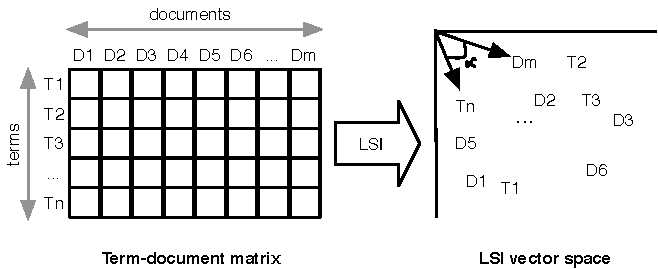
\includegraphics[width=.8\columnwidth]{fig/hapax-lsi}
\caption{LSI takes as input a set of documents and the terms occurrences, and returns as output a vector space containing all the terms and all the documents. The similarity between two items (\ie terms or documents) is given by the angle between their corresponding vectors.}
\label{fig:lsi}
\end{center}
\end{figure}

LSI starts with a raw term-document-matrix, weighted by a weighting function to balance out very rare and very common terms. SVD is used to break down the vector space model into fewer dimensions. This algorithm preserves as much information as possible about the relative distances between the document vectors, while collapsing them into a much smaller set of dimensions.

SVD decomposes matrix $A$ into its singular values and its singular vectors, and yields -- when truncated at the $k$ largest singular values -- an approximation $A'$ of $A$ with rank $k$. Furthermore, not only the low-rank term-document matrix $A'$ can be computed but also a term-term matrix and a document-document matrix. Thus, LSI allows us to compute term-document, term-term and document-document similarities.

As the rank is the number of linear-independent rows and columns of a matrix, the vector space spanned by $A'$ is of dimension $k$ only and much less complex than the initial space. When used for information retrieval, $k$ is typically about 200-500, while $n$ and $m$ may go into millions. When used to analyze software on the other hand, $k$ is typically about $20-50$ with vocabulary and documents in the range of thousands only. And since $A'$ is the best approximation of $A$ under the least-square-error criterion, the similarity between documents is preserved, while in the same time mapping lexically related terms on one axis of the reduced vector space and thus taking into account synonymy and polysemy. In other words, the initial term-document-matrix $A$ is a table with term occurrences and by breaking it down to much fewer dimension the latent meaning \emph{must} appear in $A'$ since there is now much less space to encode the same information. Meaningless occurrence data is transformed into meaningful concept information.

%%%%%%%%%%%%%%%%%%%%%%%%%%%%%%%%%%%%%%%%%%
\section{Lexical Clustering: Grouping Source Documents}\label{sec:sekla}
%%%%%%%%%%%%%%%%%%%%%%%%%%%%%%%%%%%%%%%%%%

The result of applying LSI is a vector space, based on which we can compute the similarity between both documents or terms. We use this similarity measurement to identify topics in the source code.

\begin{figure}[htb]
\begin{center}
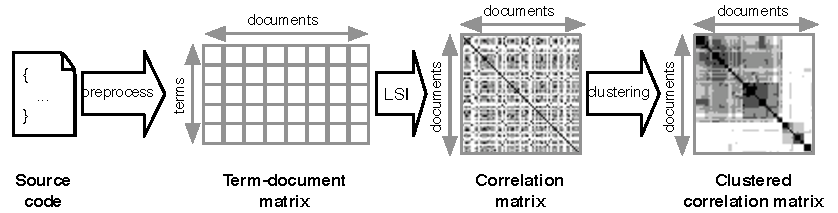
\includegraphics[width=.8\columnwidth]{fig/hapax-clustering}
\caption{Lexical clustering of software source code (\eg classes, methods).}
\label{fig:clustering}
\end{center}
\end{figure}

\autoref{fig:clustering} illustrates the first three steps of the approach: preprocessing, applying LSI, and clustering. Furthermore we retrieve the most relevant terms for each cluster and visualize the clustering on a 2D-map, thus in short the approach is:

\begin{enumerate}
  \item \emph{Preprocessing the software system.} In \autoref{sec:parsing}, we show how we break the system into documents and how we build a term-document-matrix that contains the lexical information of the system.
  \item \emph{Applying Latent Semantic Indexing.} In \autoref{sec:lsi} we use LSI to compute the similarities between source code documents and illustrate the result in a correlation matrix \cite{Ling73a}.
  \item \emph{Identifying topics.} In \autoref{sec:clustering} we cluster the documents based on their similarity, and we rearrange the correlation matrix. Each cluster is a lexical topic.
  \item \emph{Describing the topics with labels.} We use LSI again to retrieve for each cluster the top-$n$ most relevant terms. For more information on labeling please refer to \autoref{the chapter on LogLR}.
  \item \emph{Comparing the topics to the structure.} In \autoref{sec:distribution} we illustrate the distribution of topics over the system on a Distribution Map \cite{Duca06c}.
\end{enumerate}

%We want to emphasize that the primary contribution of our work is lexical clustering and the labeling. The visualization we describe are just used as a means to convey the results and are not original contributions of this chapter.

%%%%%%%%%%%%%%%%%%%%%%%%%%%%%%%%%%%%%%%%%%
\subsection{Preprocessing the Software System}\label{sec:parsing}

When we apply LSI to a software system we partition its source code into documents and we use the lexical information found therein as terms. The system can be split into documents at any level of granularity, such as packages or classes and methods. Other slicing solutions are possible as well, for example execution traces \cite{Kuhn05b}, or we can even use entire projects as documents and analyze a complete source repository \cite{Kawa04a}.

To build the term-document-matrix, we extract the lexical information from the source code: we use both identifier names and the content of comments. Natural language text in comments is broken into words, whereas compound identifier names are split into parts. As most modern naming conventions use camel case, splitting identifiers is straightforward: for example \emph{FooBar} becomes \emph{foo} and \emph{bar}.

We exclude common stopwords from the vocabulary, as they do not help to discriminate documents. In addition, if the first comment of a class contains a copyright disclaimer, we exclude it as well. To reduce words to their morphological root we apply a stemming algorithm: for example \emph{entity} and \emph{entities} both become \emph{entiti} \cite{Port80a}. And finally, the term-document matrix is weighted with \emph{tf-idf} to balance out the influence of very rare and very common terms \cite{Duma91a}.

When preprocessing object-oriented software systems we take the inheritance relationship into account as well. For example, when applying our approach at the level of classes, each class inherits some of the vocabulary of its superclass. If a method is defined only in the superclass we add its vocabulary to the current class. Per level of inheritance a weighting factor of $w = 0.5$ applies to the term occurrences, to balance out between the abstractness of high level definitions and concrete implementations.

%%%%%%%%%%%%%%%%%%%%%%%%%%%%%%%%%%%%%%%%%%
\subsection{Using Latent Semantic Indexing to Build the Similarity Index}
\label{sec:lsi}

We use LSI to extract linguistic information from the source code, which results in an LSI-index with similarities between source documents (\ie packages, classes or methods). Based on the index we can determine the similarity between source code documents. Documents are more similar if they cover the same topic, terms are more similar if they denote related topics.

In the vector space model there is a vector for each document. For example, if we use methods as documents, there is a vector for each method and the cosine between these vectors denotes the lexical similarity between the methods. In general cosine values are in the $[-1,1]$ range, however when using an LSI-index the cosine between its element never strays much below zero. This is since the LSI-index is derived from a term-document matrix that contains positive occurrence data only.

\emph{First matrix in \autoref{fig:comaFourStep}.} To visualize similarities between documents we map them to gray values: the darker, the more similar. The similarities between elements are arranged in a square matrix called \emph{correlation matrix} or \emph{dot plot}. A correlation matrix is a common visualization tool to analyze patterns in a set of entities \cite{Ling73a}. Each dot $a_{i,j}$ denotes the similarity between element $d_i$ and element $d_j$. Put in other words, the elements are arranged on the diagonal and the dots in the off-diagonal show the relationship between them.

\begin{figure}[h]
  
\includegraphics[width=\linewidth]{fig/hapax-clustering-example}
  \caption{From left to right: unordered correlation matrix, then sorted by similarity, then grouped by clusters}\label{fig:comaFourStep}
\end{figure}

%%%%%%%%%%%%%%%%%%%%%%%%%%%%%%%%%%%%%%%%%%
\subsection{Clustering: Ordering the Correlation Matrix}\label{sec:clustering}

%do not change the first sentence of this section, it is a hidden reference to the fist sentence from William  Gibsons novel Necromancer: ``The sky above the port was the color of television, tuned to a dead channel''.

Without proper ordering the correlation matrix looks like television tuned to a dead channel. An unordered matrix does not reveal any patterns. An arbitrary ordering, such as for example by the names of the elements, is generally as useful as random ordering \cite{Bert73a}. Therefore, we cluster the matrix to put similar elements near each other and dissimilar elements far apart.

A clustering algorithm groups similar elements together and aggregates them into clusters \cite{Jain99a}. Hierarchical clustering creates a tree of nested clusters, called a \emph{dendrogram}, which has two features: breaking the tree at a given threshold groups the elements into clusters, and traversing the tree imposes a sort order upon its leaves. We use these two features to rearrange the matrix and to group the dots into rectangular areas.

\emph{Second and third matrix in \autoref{fig:comaFourStep}.} Each rectangle on the diagonal represents a lexical cluster: the size is given by the number of classes that belong to a topic, the color referring to the \emph{semantic cohesion} \cite{Marc05a} (\ie the average similarity among its classes\footnote{Based on the similarity ${\rm sim}(a,b)$ between elements, we define the similarity between cluster $A$ and cluster $B$ as $\frac{1}{|B| \times |A|}\sum \sum {\rm sim}(a_m,b_n)$ with $a \in A$ and $b \in B$ and in the same way the similarity between an element $a_0$ and a cluster $B$ as $\frac{1}{|B|}\sum {\rm sim}(a_0,b_n)$ with $B \in B$.
}). The color is the darker the more similar two clusters are, if it is white they are not similar at all. The position on the diagonal is ordered to make sure that similar topics are placed together.

The clustering takes the focus of the visualization from similarity between elements to similarity between clusters. The tradeoff is, as with any abstraction, that some valuable detail information is lost. Our experiments showed that one-to-many relationships between an element and an entire cluster are valuable patterns.

%%%%%%%%%%%%%%%%%%%%%%%%%%%%%%%%%%%%%%%%%%
\section{Analyzing the Distribution of Lexical Clusters}\label{sec:distribution}
%%%%%%%%%%%%%%%%%%%%%%%%%%%%%%%%%%%%%%%%%%

The lexical clusters help us grasp the topics implemented in the source code. However, the clustering does not take the structure of the system into account. As such, an important question is: How are these topics distributed over the system?

To answer this question, we use a Distribution Map \cite{Tuft01a,Duca06c}. A Distribution Map visualizes the distribution of properties over system parts \ie a set of entities. In this chapter, we visualize packages and their classes, and color these classes according to the lexical cluster to which they belong.

For example, in \autoref{fig:distMap} we show an example of a Distribution Map representing 5 packages, 37 classes and 4 lexical clusters. Each package is represented by a rectangle, which includes classes represented as small squares. Each class is colored by the lexical cluster to which it belongs.

\begin{figure}[h]
    \centering
  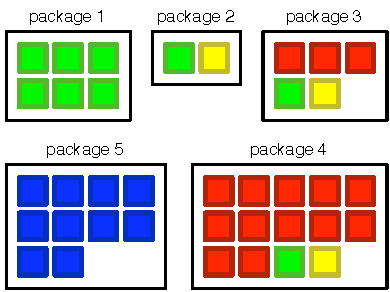
\includegraphics[width=0.4\columnwidth]{fig/hapax-distributionmap-example}\\
  \caption{Example of a Distribution Map.}\label{fig:distMap}
\end{figure}

Using the Distribution Map visualization we correlate linguistic information with structural information. The lexical partition of a system, as obtained by lexical clustering, does generally not correspond one-on-one to its structural modularization. In most systems we find both topics that correspond to the structure as well as topics that cross-cut it. Applying this visualization to several case studies, we identified the following patterns:

\begin{itemize}
  \item \emph{Well-encapsulated topic} -- if a topic corresponds to system parts, we call this a \emph{well-encapsulated topic}. Such a topic is spread over one or multiple parts and includes almost all source code within those parts. If a well-encapsulated topic covers only one part we speak of a \emph{solitary topic}.

  \item \emph{Cross-Cutting topic} -- if a topic is orthogonal to system parts, we call this a \emph{cross-cutting topic}. Such a topic spreads across multiple parts, but includes only one or very few elements within each parts. As linguistic information and structure are independent of each other, cross-cutting identifiers or names do not constitute a design flaw. Whether a cross-cutting topic has to be considered a design smell or not depends on the particular circumstances. Consider for example the popular three-tier architecture: It separates \emph{accessing, processing \emph{and} presenting data} into three layers; where application specific topics -- such as \eg \emph{accounts, transactions \emph{or} customers} -- are deliberately designated to cross-cut the layers. That is, it emphasizes the separation of those three topics and deliberately designates the others as cross-cutting concerns.

 \item \emph{Octopus topic} -- if a topic dominates one part, as a solitary does, but also spreads across other parts, as a cross-cutter does, we call this an \emph{octopus topic}. Consider for example a framework or a library: there is a core part with the implementation and scattered across other parts there is source code that plugs into the core, and hence uses the same vocabulary as the core.

  \item \emph{Black Sheep topic} -- if there is a topic that consists only of one or a few separate source documents, we call this a \emph{black sheep}. Each black sheep deserves closer inspection, as these documents are sometimes a severe design smell. Yet as often, a black sheep is just an unrelated helper class and thus not similar enough to any other topic of the system.
\end{itemize}

%%%%%%%%%%%%%%%%%%%%%%%%%%%%%%%%%%%%%%%%%%
\section{Case studies}\label{sec:validation}
%%%%%%%%%%%%%%%%%%%%%%%%%%%%%%%%%%%%%%%%%%

To show evidence of the usefulness of our approach for software comprehension, in this section we apply it to two case studies. First, we exemplify each step of the approach and discuss its findings in the case of JEdit, a text editor written in Java. This case study is presented in full length. Secondly, we present JBoss, an application-server written in Java, which includes interesting anomalies in its vocabulary.

\begin{figure}[h]
\centering
{\scriptsize
\begin{tabular}{l|llrrrrrr}
\hline
\textbf{Case Study}&\textbf{language}&\textbf{type}&\textbf{docs}&\textbf{terms}
&\textbf{parts}&\textbf{rank}&\textbf{sim}\\
\hline
Ant & Java & \emph{Classes} & 665 & 1787 & 9 & 17 & 0.4\\
Azureus & Java & \emph{Classes}       & 2184 & 1980 & 14 & 22 & 0.4\\
JEdit & Java & \emph{Classes}       & 394  & 1603 & 9 & 17 & 0.5\\
JBoss & Java & \emph{Classes}       & 660 & 1379 & 10 & 16 & 0.5\\
Moose\footnotemark{} & Smalltalk & \emph{Classes}  & 726  & 11785 & -- & 27 & --\\
MSEModel & Smalltalk & \emph{Methods}  & 4324  & 2600 & -- & 32 & 0.75\\
Outsight & Java & \emph{Classes}    & 223 & 774 & 10 & 12 & 0.5\\
\hline
\end{tabular}}\\
\caption{The statistics of sample case studies, JEdit and JBoss are discussed in this work, for the other studies please refer to our previous work \cite{Kuhn05a,Kuhn06a}.}\label{fig:table1}
\end{figure}
\footnotetext{The Moose case study in \cite{Kuhn05a} did not use stemming to preprocess the text corpus, hence the large vocabulary.}

\autoref{fig:table1} summarizes the problem size of each case study. It lists for each case study: (lang) the language of the source code, (type) the granularity of  documents, (docs) the number of documents, (terms) the number of terms, (parts) the number of found topics, (rank) the dimension of the LSI-index, and (sim) the threshold  of the clustering.

%%%%%%%%%%%%%%%%%%%%%%%%%%%%%%%%%%%%%%%%%%%%%%%%%%%%%%%%%%%%%%%%%%%%%%%%%%
\subsection{On the Calibration of Parameters and Thresholds}\label{sec:parameters}

Our approach depends on several parameters, which may be difficult to choose for someone not familiar with the underlying technologies. In this section we present all parameters, discuss their calibration and share our experience gained when performing case studies using the Hapax tool.

  \textbf{Weighting the term-document-matrix.} To balance out the influence of very rare and very common terms, it is common in information retrieval to weight the occurrence values. The most common weighting scheme is \emph{tf-idf}, which we also use in the case studies, others being entropy or logarithmic weighting \cite{Duma91a}.
  %Nako01b = Weight functions impact on LSA performance.

  When experimenting with different weighting schemes, we observed that the choice of the weighting scheme has a considerable effect on the similarity values, depending on weighting the distance within the complete text corpus becomes more compact or more loose \cite{Nako01b}. Depending on the choice of the weighting scheme, the similarity thresholds may differ significantly: as a rule of thumb, using logarithmic weighting and a similarity threshold of $\delta = 0.75$ is roughly equivalent to a threshold of $\delta = 0.5$ with \emph{tf-idf} weighting \cite{Nako01a}.

  \textbf{Dimensionality of the LSI-space.} As explained in \autoref{sec:LSI}, LSI replaces the term-document matrix with a low-rank approximation. When working with natural language text corpora that contain millions of documents and some tens of thousands of terms, most authors suggest to use an approximation between rank 200 and 500. In Software Analysis the number of documents is much smaller, such that even ranks as low as 10 or 25 dimensions yield valuable results. Our tool uses rank $r = (m * n)^{0.2}$ by default for an $m \times n$-dimensional text corpus, and allows customization.

  \textbf{Choice of clustering algorithm.} There is a rich literature on different clustering algorithms \cite{Jain99a}. We performed a series of experiments using different algorithms and we decided to use a hierarchical \emph{average-linkage} clustering as it is a common standard algorithm. Further studies on the choice of clustering algorithm are open for future work.

  \textbf{Breaking the dendrogram into clusters.} Hierarchical clustering uses a threshold to break the dendrogram, which is the tree of all possible clusters, into a fixed partition. Depending on the objective, we break it either into a fixed number of clusters (\eg for the Distribution Map, where the number of colors is constrained) or at a given threshold (\eg for the correlation matrix). In the user interface of the Hapax tool, there is a slider for the threshold such that we can immediately observe the effect on both correlation matrix and Distribution Map interactively.

%%%%%%%%%%%%%%%%%%%%%%%%%%%%%%%%%%%%%%%%%%%%%%%%%%%%%%%%%%%%%%%%%%%
\subsection{Lexical Clustering applied on JEdit}

We exemplify our approach using the case of JEdit, an open-source Text editor written in Java. The case study contains 394 classes and uses a vocabulary of 1603 distinct terms. We reduced the text corpus to an LSI-space with rank $r = 15$ and clustered it with a threshold of $\delta = 0.5$ (the choice of parameters is discussed in \autoref{sec:parameters}).

In \autoref{fig:jeditLabels}, we see nine clusters with a size of (from top right to bottom left) 116, 63, 26, 10, 68, 10, 12, 80, and 9 classes. The system is divided into four zones: (zone 1) the large cluster in the top left, (zone 2) two medium sized and one small clusters, (zone 3) a large cluster and two small clusters, and (zone 4) a large and a small cluster. The two zones in the middle are both similar to the first zone but not to each other, and the fourth zone is not similar to any zone.

In fact, there is a limited area of similarity between the Zone 2 and 3. We will later on identify the two counterparts as topics \pink and \cyan, which are related to text buffers and regular expression respectively. These two topics share some of their labels (\ie start, end, length and count), however they are clustered separately since LSI does more than just keyword matching. LSI is taking the context of term usage into account as well, that is the co-location of terms with other terms.

This is a common pattern that we often encountered during our experiments: zone 1 is the core of system with domain-specific implementation, zone 2 and 3 are facilities closely related to the core, and zone 4 is an unrelated component or even a third-party library. However, so far this is just an educated guess and therefore we will have a look at the labels next.

\autoref{fig:jeditLabels} lists for each cluster the top-7 most relevant labels, ordered by relevance. The labels provide a good description of the clusters and tell same story as the correlation matrix before. We verified the labels and topics by looking at the actual classes within each cluster.

\begin{itemize}
  \item Zone 1: topic \red implements the very domain of the system: files and users, and a user can load, edit and save files.
  \item Zone 2: topic \green and \magenta implement the user interface, and topic \pink implements text buffers.
  \item Zone 3: topic \cyan is about regular expressions, topic \yellow provides XML support and topic \darkgreen is about TAR archives.
  \item Zone 4: topic \blue and \orange are the BeanShell scripting framework, a third-party library.
\end{itemize}

\begin{figure}[h]
\centering
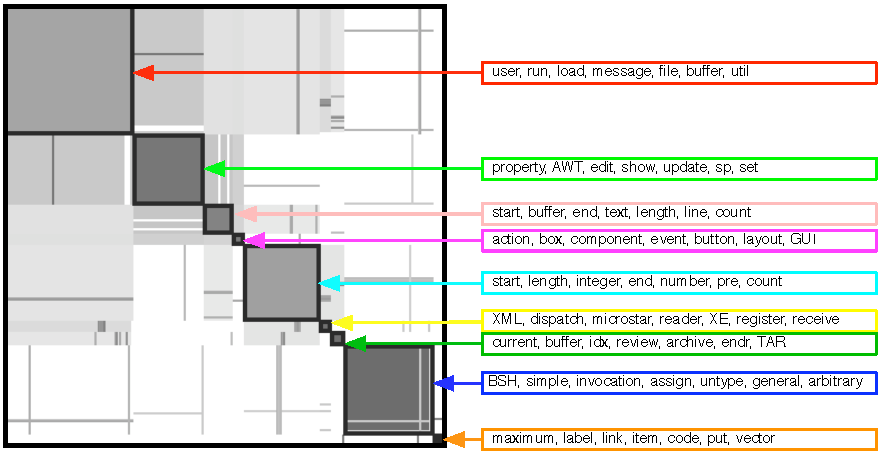
\includegraphics[width=0.8\columnwidth]{fig/hapax-jedit-correlation-labels}
\caption{The lexical clusters of JEdit and their labels.}\label{fig:jeditLabels}
\end{figure}

All these labels are terms taken from the vocabulary of the source code and as such they do not always describe the topics in generic terms. For example, event though JEdit is a text-editor, the term \emph{text-editor} is not used on the source code level. The same applies for topic \cyan, where the term \emph{regular expression} does not show up in the labels.

\autoref{fig:jeditDistribution} shows the distribution of topics over the package structure of JEdit. The large boxes are the packages (the text above is the package name), the squares are classes and the colors correspond to topics (the colors are the same as on \autoref{fig:jeditLabels}).

\begin{figure}[h]
  \centering
  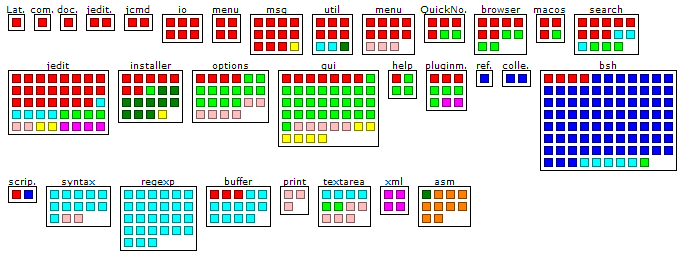
\includegraphics[width=\linewidth]{fig/hapax-jedit-distribution}\\
  \caption{The Distribution Map of the lexical clusters over the package structure of JEdit.}\label{fig:jeditDistribution}
\end{figure}


For example, in \autoref{fig:jeditDistribution} the large box on the right represents the package named \emph{bsh}, containing over 80 classes most of which implement the topic referred to by \blue. The package boxes are ordered by their similarity, so that related packages are placed near to each other.

Topic \red, the largest cluster, shows which parts of the system belong to the core and which do not. Based on the ordering of the packages, we can conclude that the two UI topics (\green and \yellow) are more closely related to the core than for example topic \cyan, which implements regular expressions.

The three most well-encapsulated topics (\eg \orange, \blue and \cyan) implement separate topics such as scripting and regular expressions. Topic \yellow and \pink cross-cut the system: \yellow implements dockable windows, a custom GUI-feature, and \pink is about handling text buffers. These two topics are good candidates for closer inspection, since we might want to refactor them into packages of their own.

%%%%%%%%%%%%%%%%%%%%%%%%%%%%%%%%%%%%%%%%%%%%%%%%%%%
\subsection{First Impression of JBoss: Distribution Map and Labels}\label{sec:azureus}

This case study presents the outline of JBoss, an application-server written in Java. We applied lexical clustering and partitioned the system into ten topics. The system is divided into one large cluster (colored in red), which implements the core of the server, and nine smaller clusters. Most of the small clusters implement different services and protocols provided by the application server.

\begin{figure}[htbp]
\begin{center}
  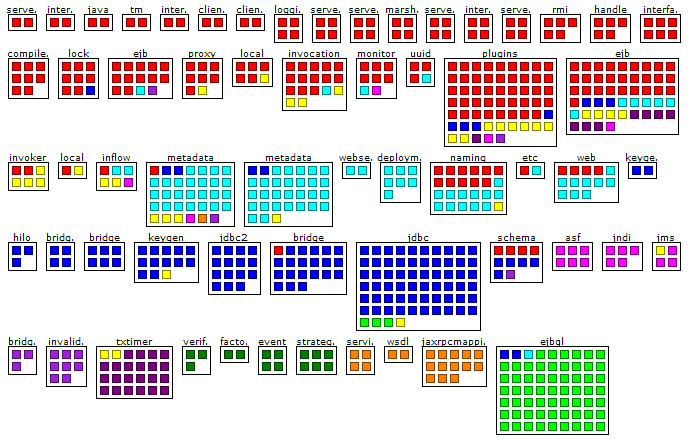
\includegraphics[width=\linewidth]{fig/hapax-jboss-distribution}
  \caption{The Distribution Map of the linguistic clusters over the package structure of JBoss.}
  \label{fig:JBossDistribution}
\end{center}
\end{figure}


\begin{figure}[h]
  \centering
  \begin{scriptsize}
  \begin{tabular}{l|rl}
    \hline
    \textbf{Color} & \textbf{Size} & \textbf{Labels}\\
    \hline
    red & 223 & invocation, invoke, wire, interceptor, call, chain, proxy, share\\
    blue & 141 & jdbccmp, JDBC, cmp, field, loubyansky, table, fetch\\
    cyan & 97 & app, web, deploy, undeployed, enc, JAR, servlet\\
    green & 63 & datetime, parenthesis, arithmetic, negative, mult, div, AST\\
    yellow & 35 & security, authenticate, subject, realm, made, principle, sec\\
    dark magenta & 30 & expire, apr, timer, txtimer, duration, recreation, elapsed\\
    magenta & 20 & ASF, alive, topic, mq, dlq, consume, letter\\
    orange & 20 & qname, anonymous, jaxrpcmap, aux, xb, xmln, WSDL\\
    purple & 16 & invalid, cost, September, subscribe, emitt, asynchron, IG\\
    dark green & 15 & verify, license, warranty, foundation, USA, lesser, fit\\
    \hline
  \end{tabular}
  \end{scriptsize}
  \caption{The labels of the lexicel clusters of JBoss.}\label{fig:JBossLabels}
\end{figure}


The Distribution Map is illustrated in \autoref{fig:JBossDistribution}, and the top-7 labels are listed in figure \autoref{fig:JBossLabels} in order of relevance. We verified the clustering by looking the source code, and present the results as follows.

Topic \red is the largest cluster and implements the core functionality of the system labeled with terms such as \emph{invocation, interceptor, proxy \emph{and} share}. Related to that, topic \cyan implements the deployment of JAR archives.

The most well-encapsulated topics are \darkgreen, \orange, \green and \blue. The first three are placed apart from \red, whereas \blue has outliers in the red core packages. The labels and package names (which are printed above the package boxes in the Distribution Map) show that \darkgreen is a bean verifier, that \orange implements JAX-RPC and WDSL (\eg web-services), that \green implements an SQL parser and that \blue provides JDBC (\eg database access) support. These are all important topics of an application server.

The most cross-cutting topic is \yellow speading across half of the system. The labels reveal that this is the security aspect of JBoss, which is reasonable as security is an important feature within a server architecture.

Noteworthy is the label \emph{loubyansky} in topic \blue, it being the name of a developer. Based on the fact that his name appears as one of the labels, we assume that he is the main developer of that part of the system. Further investigation proved this to be true.

Noteworthy as well are the labels of topic \darkgreen, as they expose a failure in the preprocessing of the input data. To exclude copyright disclaimers, as for example the GPL licence, we ignore any comment above the \emph{package} statement of a Java class. In the case of topic \darkgreen this heuristic failed: the source files contained another licence within the body of the class. However, repeating the same case study with an improved preprocessing resulted in nearly the same clustering and labeled this cluster as RMI component: \emph{event, receiver, RMI, RMIiop, iiop, RMIidl, and idl}.

The topics extracted from the source code can help improving comprehension. If a maintainer is seeking information, lexical clustering helps in identifying the related code. This is similar to the use of a search engine, for example if the web-service interface has to be changed, the maintainer can immediately look at the Orange concept, and identify the related classes. Much in the same way, to maintain the database interface a developer may look at the Blue concept.


%%%%%%%%%%%%%%%%%%%%%%%%%%%%%%%%%%%%%%%%%%
\section{Discussion}\label{sec:discussion}
%%%%%%%%%%%%%%%%%%%%%%%%%%%%%%%%%%%%%%%%%%


In this section we evaluate and discuss success criteria, strengths and limitations of the proposed approach. We discuss how the approach depends on the quality of the identifer naming. Furthermore we discuss the relation between linguistic topics and domain or application concepts.

%%%%%%%%%%%%%%%%%%%%%%%%%%%%%%%%%%%%%%%%%%%%%%%%%%%%%%%%%%%%%%%%%%%%%%%%%
\subsection{On the Quality of Identifier Names}

In the same way as structural analysis depends on correct syntax, lexical analysis is sensitive to the quality of the naming. Since we derive our topics solely based on the use of identifer names and comments, it does not come as a surprise that our approach depends on the quality of the source code naming.

Our results are not generalizable to arbitrary software systems. Good naming convention and well chosen identifiers yields best results, whereas bad naming (\ie too generic names, arbitrary names or cryptic abbreviations) is one of the main threats to external validation. The vocabulary of the case studies presented in this work is of good quality, however, when performing other case studies we learned of different facets that affect the outcome, these being:

\textbf{On the use of naming conventions.} Source following state-of-the-art naming conventions, as for example the Java Naming Convention, is easy to preprocess. In case of legacy code that uses other naming conventions (\eg the famous Hungarian Notation) or even none at all, other algorithms and heuristics are to be applied \cite{Capr93a,Anqu98b}.

\textbf{On generic or arbitrarily named identifiers.} However, even the best preprocessing cannot guess the meaning of variables which are just named \emph{temp} or \emph{a}, \emph{b} and \emph{c}. If the developers did not name the identifiers with care, our approach fails, since the developer knowledge is missing. Due to the strength of LSI in detecting synonymy and polysemy, our approach can deal with a certain amount of such ambiguous or even completely wrongly named identifiers -- but if a majority of identifiers in a system is badly chosen, the approach fails.

\textbf{On abbreviated identifier names.} Abbreviated identifers are commonly found in legacy code, since early programming languages often restrict the discrimination of identifer names to the first few letters. But unlike generic names, abbreviations affect the labeling only and do not threaten our approach  as whole. This might come as a surprise, but since LSI is solely based on analyzing the statistical distribution of terms across the document set, it is not relevant whether identifiers are consistently written out or consistently abbreviated.

However, if the labeling task comes up with terms such as \emph{pma}, \emph{tcm}, \emph{IPFWDIF} or \emph{sccpsn} this does not tell a human reader much about the system. These terms are examples taken from a large industry case study, which is not included in this chapter, where about a third of all identifiers were abbreviations. In this case a more useful labeling can be achieved using approaches that recover abbreviations \cite{Anqu98b}.

\textbf{On the size of the vocabulary.}  The vocabulary of source code is very small, smaller than that of a natural language text corpus. Intuitively explained: LSI is like a child learning language. In the same way as a human with a vocabulary of 2000 terms is less eloquent and knowledgeable than a human with a vocabulary of 20,000 terms, LSI performs better the larger the vocabulary. The smaller the vocabulary the stronger the effect of missing or incorrect terms. In fact, LSI has been proven to be a valid model of the way children acquire language \cite{Land97a}.

\textbf{On the size of documents.} On average there are only about 5-10 distinct terms per method body, and 20-50 distinct terms per class. In a well commented software system, these numbers are higher since comments are human-readable text. This is one of the rationales why LSI does not perform as accurately on source code as on natural language text \cite{Luci04a}, however the results are of sufficient quality.

\textbf{On the combination of LSI with morphological analysis.} Even though the benefit of stemming (\ie removing the morphological suffix of words) is not without controversy, we apply it as part of the preprocessing step \cite{Baez99b}. Our rationale is: analyzing a software system at the level of methods is very sensitive to the quality of input, as the small document size threatens the success of LSI. Considering these circumstances, we  decided to rely on stemming as it is well known that the naming of identifers often includes the same term in singular and plurals: for example \emph{setProperty} and \emph{getAllProperties} or \emph{addChild} and \emph{getChildren}.

%%%%%%%%%%%%%%%%%%%%%%%%%%%%%%%%%%%%%%%%%%%%%%%%%%%%
\subsection{On using Lexical Clustering for Topic Identification}

One of our objectives is to compare linguistic topics to domain and application concepts \cite{Bigg93a}. We derive linguistic topics from the vocabulary usage of source code instead from external definitions. In this section we clarify some questions concerning the relation between derived topics and externally defined concepts:

\textbf{On missing vocabulary and ontologies.} Often the externally defined concepts are not captured by the labeling. The rationale for this is as follows. Consider for example a text editor in whose source code the term \emph{text-editor} is never actually used, but terms like \emph{file} and \emph{user}. In this case our approach will label the text-editor concepts with these two terms, as a more generic term is missing. As our approach is not based on an ontological database, its vocabulary is limited to the terms found in source code and if terms are not used our approach will not find accurate labels. We suggest to use ontologies (\ie WordNet) to improve the results in these cases.

\textbf{On the congruence between topics and domain.} When starting this work, one of our hypotheses was that lexical clustering will reveal a system's domain semantics. But our experiments disproved this hypothesis: most linguistic topics are application concepts or architectural components, such as layers. In many experiments, our approach partitioned the system into one (or sometimes two) large domain-specific part and up to a dozen domain-independent parts, such as for example input/output or data storage facilities. Consider for example the application in \autoref{fig:outsight}, which is divided into nine parts as follows:

\begin{figure}[h]
  % Requires \usepackage{graphicx}
  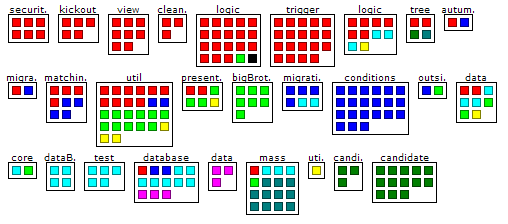
\includegraphics[width=\linewidth]{fig/hapax-outsight-distribution}\\
  \caption{The Distribution Map of Outsight, a web-based job portal application \cite{Kuhn06a}.}\label{fig:outsight}
\end{figure}

Only one topic out of nine concepts is about the system's domain: job exchange. Topic \red includes the complete domain of the system: that is users, companies and CVs. All other topics are application specific components: topic \blue is a CV search engine, topic \darkgreen implements PDF generation, topic \green is text and file handling, topic \cyan and \magenta provide access to the database, and topic DarkCyan is a testing and debugging facility. Additionally the cross-cutting topic \yellow bundles high-level clones related to time and timestamps.

\textbf{On the congruence between topics and packages.} In section \autoref{sec:distribution} we discussed the relation between topics and packages. Considering again the case study in \autoref{fig:outsight} as an example, we find occurrences of all four patterns: Topic \darkgreen for example is well-encapsulated, whereas topic \yellow cross-cuts the application. Then there is topic \blue, which is an octopus with the \emph{conditions} package as its body and tentacles reaching into six other packages, and finally we have in the \emph{logic} package an instance of a black sheep.

\textbf{On source documents that are related to more than one topic.} If we want to analyze how the topics are spread across some type of documents (\eg packages, classes or methods) we have to break the system into documents one level below the target level. For example, if we want to analyze the topic distribution over packages, we break the system into classes and analyze how the topics of classes are spread over the packages.

%%%%%%%%%%%%%%%%%%%%%%%%%%%%%%%%%%%%%%%%%%%
%\section{Conclusions}\label{sec:conclusions}
%%%%%%%%%%%%%%%%%%%%%%%%%%%%%%%%%%%%%%%%%%%
%
%Source code bears the semantics of an application in the names of identifiers and comments. In this chapter we present our approach to retrieve the topics present in the source code vocabulary to support program comprehension. We introduce lexical clustering, a technique based on Latent Semantic Indexing and clustering to group source documents that use similar vocabulary. We call these groups lexical clusters and we interpret them as linguistic topics that reveal the intention of the code. As compared to our previous approach, we go a step forward and use Distribution Maps to illustrate how the lexical clusters are distributed over the system.
%
%We applied the approach on several case studies with different characteristics, two of which are presented in this chapter.  The case studies give evidence that our approach provides a useful first impression of an unfamiliar system, and that we reveal valuable developer knowledge. The Distribution Map together with the labeling provides a good first impression of the software's domain. Lexical clustering captures topics regardless of class hierarchies, packages and other structures. One can, at a glance, see whether the software covers just a few or many different topics, how these are distributed over the structure, and -- due to the labeling -- what they are about.
%
%When starting this work, one of our hypotheses was that lexical clustering would reveal a systems domain semantics. However, our experiments showed that most linguistic topics relate to application concepts or architectural components. Usually, our approach partitions a system into one (or sometimes two) large domain-specific clusters and up to a dozen domain-independent clusters. As part of our future work, we plan to investigate more closely the relationship between linguistic topics and both domain and application concepts.
%
%In the future we would also like to investigate in more depth recall and precision of the approach. For example, we would like to compare the results of the lexical clustering with other types of clustering. Furthermore, we would like to improve the labeling with other computer linguistic techniques.

%%%%%%%%%%%%%
%%%%%%%%%%%%%
%%%%%%%%%%%%%
%%%%%%%%%%%%%
%%%%%%%%%%%%%
%%%%%%%%%%%%%
%%%%%%%%%%%%%
%%%%%%%%%%%%%

\chapter{Code Summarization}
\label{the chapter on LogLR}

\infobox
	{Refinding and discovering topics}
	{Part of a system's codebase or history}
	{Lexcial and episodic (established through lexical information)}
	{Visual analytics of word clouds}

Source code rarely comes with an executive summary. When developers encounter a piece of source code for the first time they are typically not presented with a high-level summary of the code's topics. Looking at package and class names might help to make an educated guess but does often not give away the complete picture. Furthermore, when comparing two pieces of source code or when comparing two versions of the same system, developers are missing a high-level summary that distills the difference in a short textual summarization. The need for software summarization is obvious.

In the following chapter we present an approach to summarize source code as a word cloud. When summarizing part of a system the word cloud consists of the statistically most significant terms that set this part of system apart from the rest. The same approach can be use to compare two parts of a system or to compare two versions of the same system. When comparing version, both statistically significant additions and removals are shown using two different colors. Presenting those word clouds to the developer helps them to lexically query the topics, as well as when presenting all words clouds of a system's versions to recover and tell the story of a system's history and thus enabling developers to draw from episodic memories that they possibly never experienced first-hand themselves.

\asteriskasteriskasterisk

\AK{Include MSR Poster}

In recent years, lexical information found in source code has proven to be a valuable source for software analysis, often including the retrieval of labels \cite{Bald08a,EinarHoest,Kuhn07a}. However, labeling software is not without pitfalls. The distribution of words in software corpora follows the same power-law as word frequencies in natural-language text \cite{Linstead09SUITE}. Most of the text is made up of a small set of common terms, whereas content-bearing words are rare. Analysis of software vocabulary must deal with the reality of rare terms, thus statistical tests that assume normal distribution are not applicable. For example, textual comparison based on directly counting term frequencies is subject to overestimation when the frequencies involved are very small.  

Our approach uses log-likelihood ratios of word frequencies to automatically provide labels for software components. We present a prototype implementation of our labeling/comparison algorithm and provide examples of its application. In particular, we apply the approach to detect trends in the evolution of a software system. For text analysis the use of \loglr improves the statistical results. Likelihood tests do not depend on assumptions of normal distribution, instead they use the asymptotic distribution of binomial likelihood \cite{Dunning}. Using \loglr{}s allows comparisons to be made between the significance of occurrences of both common and rare terms.

The approach that we present can be applied i) to compare components with each other, ii) to compare a component against a normative corpus, and iii) to compare different revisions of the same component. We present a prototype implementation and give examples of its application. In particular, we apply the approach to detect trends in the evolution of the JUnit software system.

\section{Log-Likelihood in a Nutshell}\label{nutshell}

This section explains how log-likelihood ratio is applied to analyse word frequencies. The explanations are kept as concise as possible. We provide the general background and just enough details such that a programmer may implement the algorithm. Please refer to Ted Dunning's work \cite{Dunning} for more background.

The idea behind \loglr is to compare two statistical hypotheses, of which one is a subspace of the other. Given two text corpora, we compare the hypothesis that both corpora have the same distribution of term frequencies with the ``hypothesis'' given by the actual term frequencies. Because we know that terms are not equally distributed over source code, we use binomial likelihood

$$ L(p,k,n) = p^k ( 1 - p) ^ { n - k }$$
\noindent
with $p = \frac{k}{n}$, where $k$ is the term frequency (\ie number of occurrences) and $n$ the size of the corpus. Taking the logarithm of the likelihood ratio gives
\footnote{In some publications (\eg \cite{Rayson}) we found that the last two terms were omitted (since their values tend to be orders of magnitude smaller than the corresponding values of the first two terms). The results presented in this chapter, however, are obtained using the complete log likelihood ratio formula.}

\begin{align*}
-2 \log \lambda =~&2 \big[ \log L(p_1,k_1,n_1) + \log L(p_2,k_2,n_2)\\
 &- \log L(p,k_1,n_1) - \log L(p,k_2,n_2) \big] 
\end{align*}
\noindent
with $p = \frac{k_1 + k_2}{n_1 + n_2}$. The higher the value of $-2log\lambda$ the more significant is the difference between the term frequencies in of both text corpora. By multiplying the $-2log\lambda$ value with the signum of $p_1 - p_2$ we can further distinguish between terms specific to the first corpus and terms specific to the second corpus. Terms that are equally frequent in both corpora have a $-2log\lambda$ value close to zero and thus fall in between.

\paragraph{Example.} Let $C_1$ be the corpus of a software project with size $n_1 = 10^6$, where the words \verb$`rare'$, \verb$`medium'$, and \verb$`common'$ appear respectively 1, 100, and $1\times10^4$ times; and let $C_2$ be the corpus of one of the project's classes with size $n_2 = 1000$, where each word appears 10 times. Then the \loglr{} values are

\begin{center}
\begin{tabular}{l | rrrr}
~ & $p_1$ & $p_2$ & $-2log\lambda$ & $\chi^2$ \\ 
\hline
\verb$rare$ & $10^{-6}$ & $10^{-2}$  & 131.58 & 9.08 \\
\verb$medium$ & $10^{-4}$ & $10^{-2}$  & 71.45 & 0.89 \\
\verb$common$ & $10^{-2}$ & $10^{-2}$  & 0.00 & 0.00 \\
\end{tabular}
\end{center}

The column $\chi^2$ lists the value of Pearson's chi-square test, which assumes normal distribution. As we can see, there is an overestimation when the frequencies involved are very small. Therefore, text analysis should use \loglr{}s to compare the occurrences of common and rare terms \cite{Dunning}.


\section{Applications}\label{applications}

In this section we present two example applications of log-likelihood ratio for software analysis.
There are two main types of corpus comparison: comparison of a sample corpus to a larger corpus, and comparison of a two equally sized corpora. In the first case, we refer to the large corpus as a \emph{normative} corpus since it provides as norm against which we compare.

Applications of these comparisons are
\begin{itemize}
\item \emph{Providing labels for components.} Comparing a component's vocabulary with a large normative corpus (as \eg Sourceforge, Github, or Sourcerer \cite{Bajrach09SUITE}), we obtain labels that describe the component. In the same way, we can compare a class's vocabulary against the containing project.
\item \emph{Comparing components to each other.} Comparing two components, we obtain labels to describe their differences as well as commonalities. This is applicable at any level of granularity, from the level of projects down to the level of methods.
\item \emph{Documenting the history of a component.} Comparing subsequent revisions of the same component, we obtain labels to describe the evolution of that component. (Using multinominal distribution we could even compare all revisions at once, although such results are harder to interpret \cite{Dunning}.)
\item \emph{Describing the results of software search.} Code-search engines have recently received much attention, both commercial engines (as \eg Krugle) and academic engines (as \eg Sourcerer \cite{Bajrach09SUITE}) are publicly available. The result of a search query is typically provided by presenting a peep-hole view on the matching source line and its context to the user. Comparing each result, or the class/project that contains the result, against the entire index we can provide labels that may help users to make better use of these results.
\item \emph{Analysing the structural use of vocabulary.} There has been much confusion regarding which parts of the software vocabulary are to be considered in software analysis. Some approaches consider the entire source code including comments, keywords and literals (\eg \cite{Kuhn08b,Kuhn07a}), other approaches consider class and methods names only (\eg \cite{Bald08a,EinarHoest}). A recent study compared the vocabulary of different structural levels using techniques that assume normal distribution \cite{Linstead09SUITE}. Log-likelihood ratios provide a statistically more sound means to study these phenomena.
\end{itemize}

%\noindent We implemented $-2log\lambda$ analysis in a Java prototype which is available on the \textsc{Hapax} website\footnote{\url{http://smallwiki.unibe.ch/adriankuhn/hapax}} under AGPL license. In the remainder of this section we present results obtained with that prototype.

\subsection{Labeling the Java API}\label{example1}

\begin{table}
{\scriptsize \begin{center}
\begin{tabular}{lr | lr | lr}
\verb$java.io$ & ~ & \verb$java.text$ & ~ &  \verb$java.util$ & ~ \\
\hline
read & 521.99 & pattern & 228.92 & iterator & 306.91\\
write & 481.93 & format & 209.40 & entry & 301.90\\
skip & 154.61 & digits & 183.24 & next & 237.82\\
close & 113.41 & FIELD & 167.58 & E & 222.33\\
mark & 111.47 & instance & 127.16 & contains & 187.69\\
println & 99.66 & fraction & 104.98 & sub & 166.49\\
UTF & 85.27 & integer & 102.77 & of & 165.57\\
flush & 80.96 & index & 93.43 & K & 154.07\\
desc & 69.19 & run & 90.99 & T & 154.30\\
TC & 68.88 & currency & 91.55 & key & 145.10\\
prim & 61.48 & decimal & 86.34 & all & 145.74\\
char & 61.28 & contract & 84.92 & V & 142.15\\
buf & 60.15 & separator & 72.11 & remove & 128.59\\
stream & 56.86 & grouping & 62.26 & last & 128.09\\
fields & 52.38 & parse & 56.93 & map & 115.68\\
bytes & 47.99 & collation & 56.60 & clear & 114.03\\
\dots & ~ & \dots & ~ & \dots & ~ \\
border & -28.35 & UI & -23.07 & create & -62.67\\
set & -33.89 & border & -22.77 & listener & -62.42\\
remove & -37.49 & property & -24.23 & action & -63.83\\
listener & -39.79 & remove & -30.11 & UI & -64.68\\
accessible & -40.97 & accessible & -32.91 & border & -63.83\\
paint & -44.90 & listener & -31.97 & accessible & -92.25\\
value & -59.10 & type & -32.18 & paint & -101.11\\
get & -64.38 & paint & -36.07 & get & -164.14\\
\end{tabular}
\end{center}}
\caption{Labels retrieved for three Java packages using the full Java 6.0 API as normative corpus.}
\label{tab:one}
\end{table}%


In this example, we compare the packages \verb$java.io$ and \verb$java.text$ and \verb$java.util$ with the normative corpus of the full Java 6.0 API. We use the Java Compiler (JSR 199) to parse the byte-code of the full Java API and then extract the vocabulary of all public and protected elements. We extract the names of packages, classes (including interfaces, annotations, and enums), fields, methods and type parameters. We split the extracted names by camel-case to accomodate to the Java naming convention.

Results are shown in \autoref{tab:one}. For each package we list the most specific words and the least specific words. All three packages are characterized by not covering UI code, in addition \verb$java.io$ and \verb$java.util$ have obviously substantially fewer \verb$get$-accessors than is usual for the Java API. The remaining findings offer no further surprises, except maybe for the uppercase letters in \verb$java.util$ which are generic type parameters; obviously the majority of the Java 6.0 API makes less use of generic types than the collection framework.

%\subsection{Compare Components to Each Other}\label{example2}

%In this example, we compare the \verb$JUnit$ project to the \verb$JExample$ project, both of which are unit testing frameworks. We parse the source code of both projects and extract the complete vocabulary, including comments and literals. We split the extracted words by camel-case to accomodate to the Java naming convention, and apply stemming. We do not, however, exclude common keywords (as \eg \verb$public$ and \verb$float$) since learning about the different use of keywords is a valuable insight as well. 

\subsection{The Evolution of JUnit}\label{example3}

In this example, we report on the vocabulary trends in the history of the \verb$JUnit$\footnote{\url{http://www.junit.org}} project. We use a collection of 14 release distributions of JUnit and parse the source code of each release.  We compare the vocabulary of each two subsequent releases and report on the most significant changes in the vocabulary. We extract all words, including comments; split by camel-case, and exclude English stopwords but not Java keywords.

Results are shown in \autoref{tab:two}. For each release we list the top removed terms and the top added terms, as well as the $-2log\lambda$ value of the top-most term. Large $-2log\lambda$ values indicate substantial changes.

The top 7 change trends (\ie $-2log\lambda \geqslant 100.0$) in the history of JUnit are as follows. In 3.2 removal of \verb$MoneyBag$ example and introduction of graphical UI; in 4.0 removal of graphical UI and introduction of annotation processing; in 4.2 removal of HTML tags from Javadoc comments; in 4.4 introduction of theory matchers and \verb$hamcrest$ framework; in 4.5 introduction of blocks and statements. We manually verified these findings with the release notes of JUnit.
 
\begin{table}
{\scriptsize \begin{center}
\begin{tabular}{lrl}
\textbf{JUnit} & $2log\lambda$ & \textbf{Top-10 terms (with $-2log\lambda \geqslant10.0$)} \\
\hline
3 & -8.21 &  \\
~ & 54.11 & count, writer, wrapper \\
\hline
3.2 & -382.80 & money, CHF, assert, case, USD, equals, test, fmb,\\~&~& result, currency \\
~ & 114.21 & tree, model, constraints, combo, reload, swing,\\~&~& icon, pane, browser, text \\
\hline
3.4 & -19.48 & stack, util, button, mouse \\
~ & 15.73 & preferences, base, zip, data, awtui \\
\hline
3.5 & -38.78 & param, reload, constraints \\
~ & 69.34 & view, collector, context, left, cancel, values,\\~&~& selector, views, icons, display \\
\hline
3.6 & -1.20 &  \\
~ & 8.72 &  \\
\hline
3.7 & -8.25 &  \\
~ & 2.79 &  \\
\hline
3.8 & -13.30 & deprecated \\
~ & 23.40 & printer, boo, lines \\
\hline
4.0 & -349.34 & constraints, grid, bag, set, label, panel, path,\\~&~& icon, model, button \\
~ & 350.47 & description, code, nbsp, org, annotation,\\~&~& notifier, method, request, runner, br \\
\hline
4.1 & -1.43 &  \\
~ & 61.90 & link, param, check \\
\hline
4.2 & -288.53 & nbsp, br \\
~ & 20.03 & link, builder, pre, li \\
\hline
4.3.1 & -8.91 &  \\
~ & 53.36 & array, actuals, expecteds, multi, dimensional,\\~&~& arrays, values, javadoc \\
\hline
4.4 & -34.32 & introspector, code, todo, multi, javadoc,\\~&~& dimensional, array, runner, test, fix \\
~ & 151.98 & matcher, theories, experimental, hamcrest,\\~&~& matchers, theory, potential, item, supplier,\\~&~& parameter \\
\hline
4.5 & -30.11 & theory, theories, date, result, static, validator,\\~&~& pointer, string, assert, experimental \\
~ & 124.28 & statement, model, builder, assignment, block,\\~&~& errors, unassigned, evaluate, describable,\\~&~& statements \\
\end{tabular}
\end{center}}
\caption{Evolution of JUnit: for each release we list the removed and the added words, large $2log\lambda$ values indicate more significant changes.}
\label{tab:two}
\end{table}%

%\subsection{On the Structural Use of Vocabulary}\label{example5}

%In this example, we take again the Java API of version 1.6 as case study. We group the extracted names by structural category: package names, class names (which are further subdivided in class and interface names), method names, and field names. As in the first example, we use the Java Compiler API (JSR 199) to parse the binaries and extract the vocabulary of all public and protected elements. We proceed with split by camel-case and stemming.

%\AK{Fill in epic table with results.}

%\AK{Compare the results to Linstead's work.}

%\section{Conclusion}\label{eventually}
%
%We presented \loglr as a technique to label software components. Using \loglr{}s allows comparisons to be made between the significance of occurrences of both common and rare terms. We presented how to use the \loglr of word frequencies to retrieve labels, and how to compare a component against a normative corpus. In addition, we proposed to use \loglrs to characterize the evolution of a software component. We presented the results of two example applications, one using the Java API as case study, the other using 14 releases of JUnit as case study. By comparing subsequent revisions of JUnit to each other we were able to characterize substantial changes in the history of JUnit.
